\chapter{Anexo I - Pliego de condiciones}
\label{ch:anexoPliegoCondiciones}

Siguiendo la recomendación oficial de la \gls{uah} sobre \gls{tfm}s, se añade el presente anexo para establecer las condiciones materiales de los diferentes equipos que han sido necesarios para desarrollar el proyecto. Se pretende garantizar que se obtengan los mismos resultados en el caso de querer replicar las diferentes pruebas realizadas en el proyecto.

\section{Condiciones materiales y equipos}

A continuación, se indican todos los equipos empleados en el desarrollo de este \gls{tfm} y sus especificaciones de \textit{software}. 

\subsection{Especificaciones Máquina A} %MI ORDENADOR
% \label{maquina_A}
% \begin{itemize}
%     \item Procesador: i7-8700K (12) @ 4.700GHz
%     \item Memoria: 15674MiB
%     \item Gráfica: Intel UHD Graphics 630
%     \item Sistema operativo: Ubuntu 20.04.6 LTS x86\_64
% \end{itemize}
% \begin{figure}[ht!]
%     \centering
%     \includegraphics[width=8cm]{archivos/img/anexos/maquinaA.png}
%     \caption{Especificaciones de la máquina A}
%     \label{fig:maquinaA}
% \end{figure}


\subsection{Especificaciones Máquina B}
% \label{maquina_B}
% \begin{itemize}
%     \item Procesador: Intel i5-7500 (4) @ 3.800GHz
%     \item Memoria: 31984MiB
%     \item Gráfica: Intel HD Graphics 630
%     \item Sistema operativo: Ubuntu 22.04.2 LTS x86\_64
% \end{itemize}
% \begin{figure}[ht!]
%     \centering
%     \includegraphics[width=8cm]{archivos/img/anexos/maquinaB.png}
%     \caption{Especificaciones de la máquina B}
%     \label{fig:maquinaB}
% \end{figure}


\subsection{Especificaciones Máquina C}
% \label{maquina_C}
% \begin{itemize}
%     \item Procesador: Intel(R) Core(TM) 12th Gen i7-1260P (16) CPU @ 4.70Ghz
%     \item Memoria: 15674MiB
%     \item Gráfica: Intel Alder Lake-P
%     \item Sistema operativo: Ubuntu 22.04.2 LTS x86\_64
% \end{itemize}
% \begin{figure}[ht!]
%     \centering
%     \includegraphics[width=8cm]{archivos/img/anexos/maquinaC.png}
%     \caption{Especificaciones de la máquina C}
%     \label{fig:maquinaC}
% \end{figure}

\subsection{Especificaciones Máquina D}





\section{Virtualización del sistema operativo Linux}
Adicionalmente, es preciso indicar que se ha empleado una máquina virtual con un sistema operativo Linux para ejecutar la herramienta \gls{brite} en la máquina A. En este caso, se ha utilizado como plataforma VMWare\footnote{https://www.vmware.com/es/products.html} y una versión del sistema operativo Ubuntu 20.04.1 LTS como se puede visualizar en la Figura \ref{fig:ubuntu}.

\begin{figure}[h!]
    \centering
    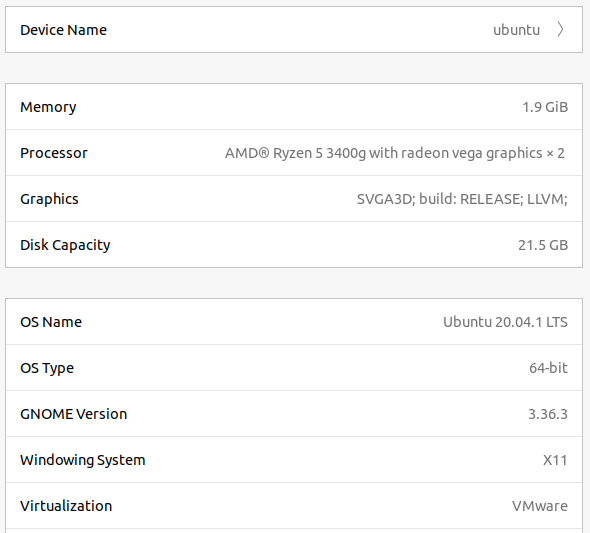
\includegraphics[width=0.75\textwidth]{img/anexos/ubuntu.PNG}
    \caption{Características del sistema operativo}
    \label{fig:ubuntu}
\end{figure}